

\subsection{Research scenario 4 results analysis}

The following figures illustrate the aggregated results from the experiments conducted within Research scenario 4 described in Chapter \ref{chap:research_scenarios}.

\begin{figure}[H]
    \begin{minipage}{.48\textwidth}
        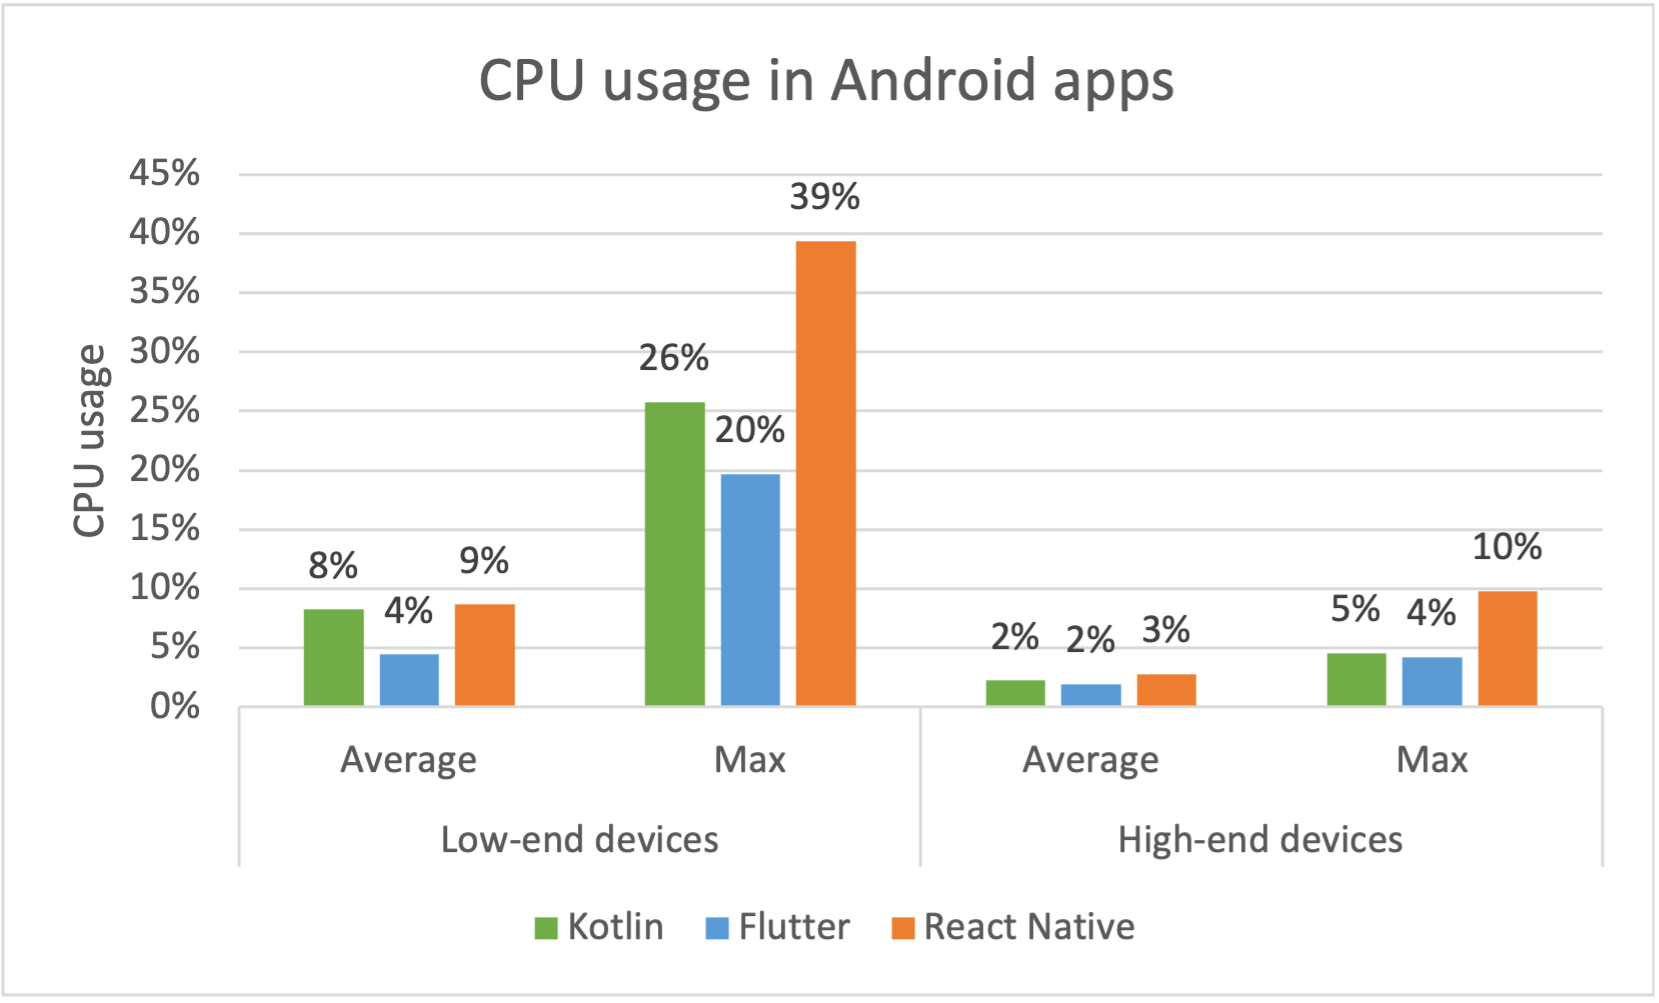
\includegraphics[width=\textwidth]{img/scenario4_cpu_android}
        \caption{Research scenario 4: CPU usage in Android apps (Source: Own work)}
        \label{fig:s4_cpu_android}
    \end{minipage}
    \hfill
    \begin{minipage}{.48\textwidth}
        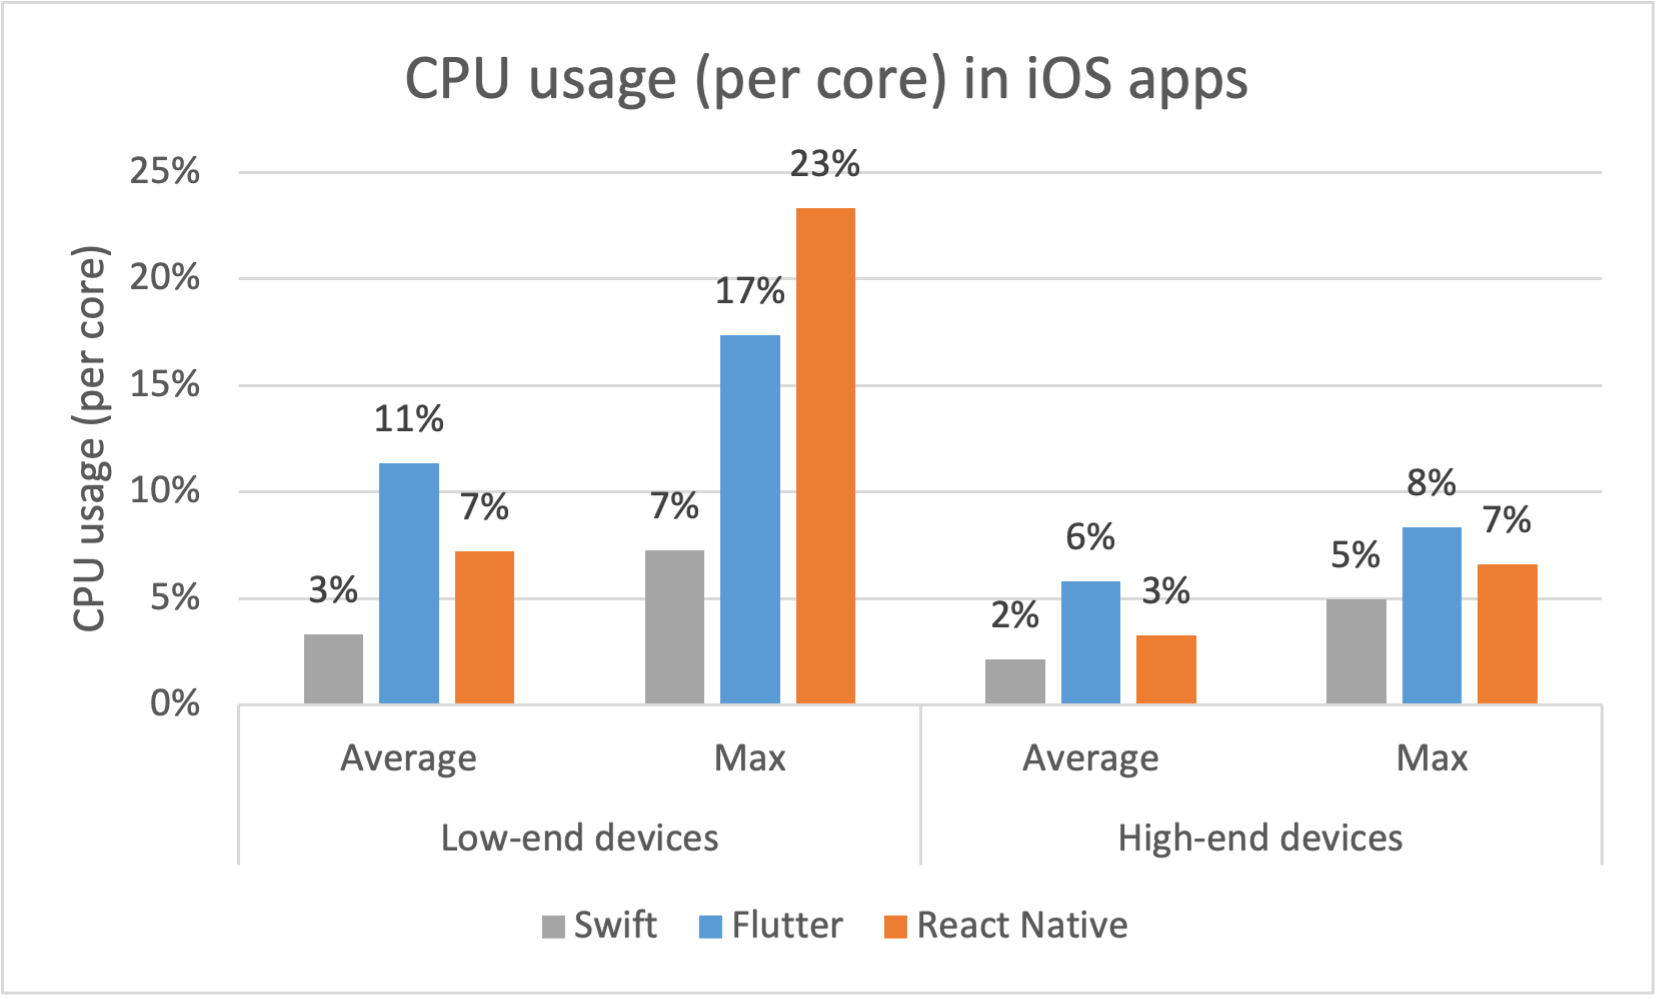
\includegraphics[width=\textwidth]{img/scenario4_cpu_ios}
        \caption{Research scenario 4: CPU usage in iOS apps (Source: Own work)}
        \label{fig:s4_cpu_ios}
    \end{minipage}
\end{figure}

Figures \ref{fig:s4_cpu_android} and \ref{fig:s4_cpu_ios} show the comparison of CPU usage among Android and iOS apps developed with Kotlin, Swift, Flutter, and React Native. On both platforms, the three technologies considered demonstrate similar CPU usage within the threshold of 2-10\% on high-end devices. On low-end Android devices, Flutter requires the least CPU capacity, while Kotlin and React Native achieve similar results, although React Native experiences higher spikes. Apps written in Swift exhibit the lowest CPU load on lower-end iOS devices. On average, React Native apps utilize less CPU resources than Flutter; however, they suffer from lower stability with spikes of 23\%.

\begin{figure}[H]
    \centering
    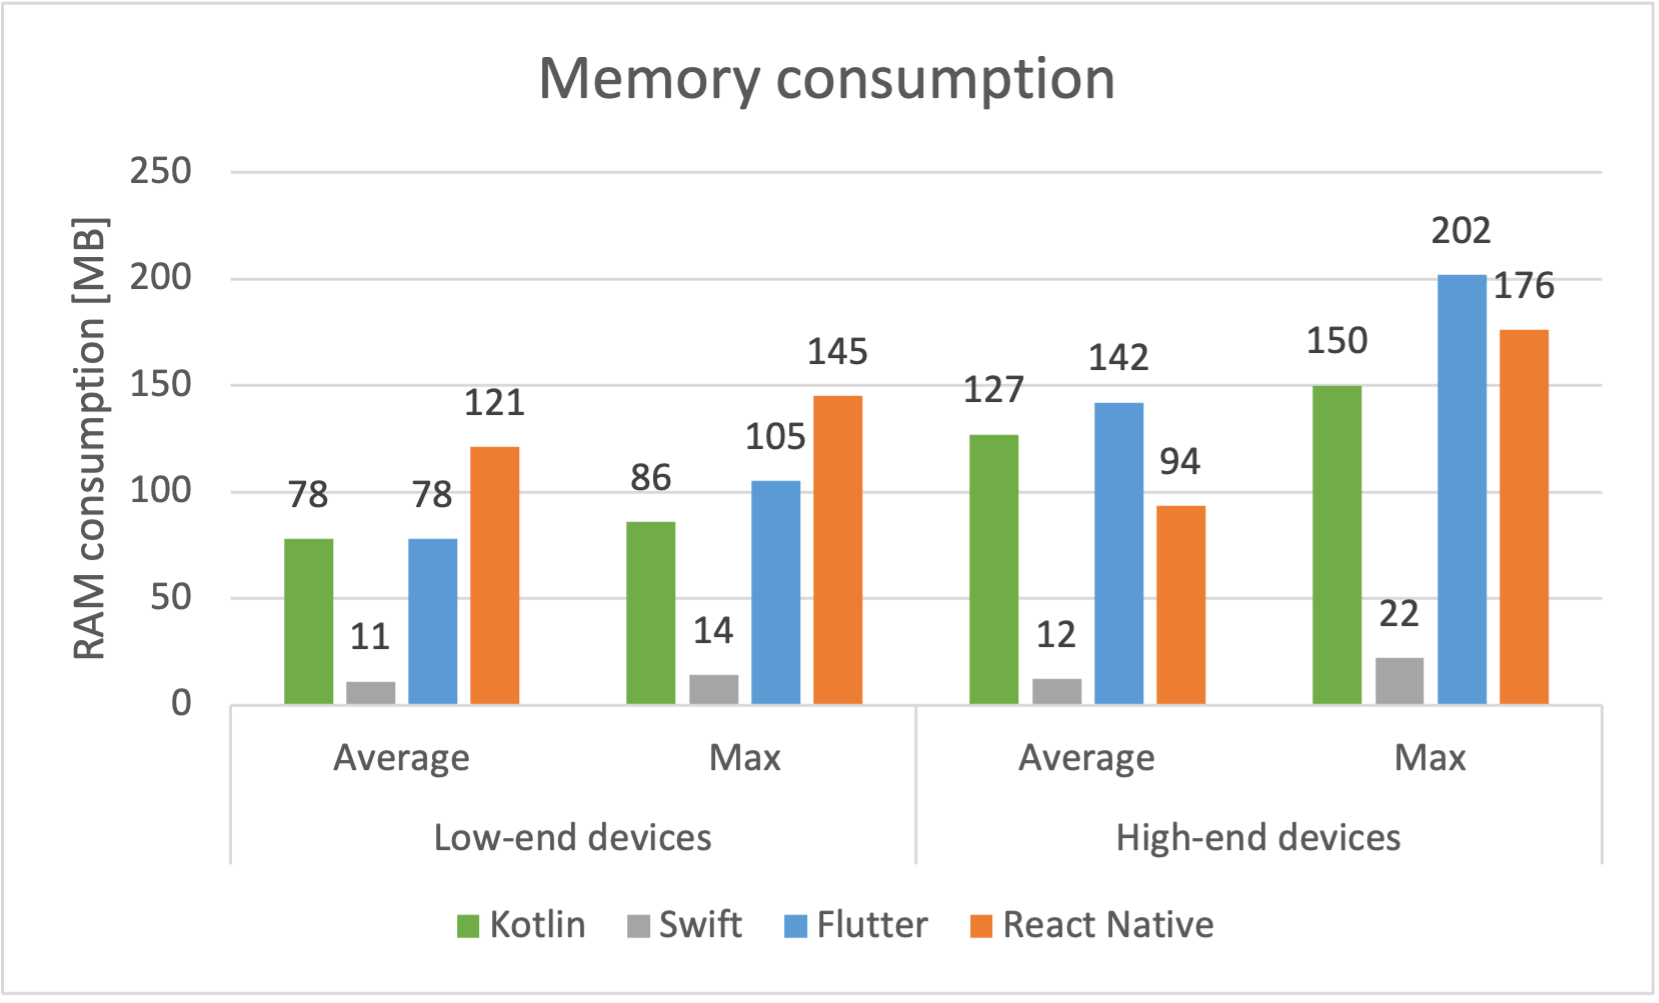
\includegraphics[width=.6\textwidth]{img/scenario4_ram}
    \caption{Research scenario 4: Memory consumption (Source: Own work)}
    \label{fig:s4_ram}
\end{figure}

Figure \ref{fig:s4_ram} shows the comparison of memory consumption among Android and iOS apps developed with Kotlin, Swift, Flutter, and React Native. It can be observed that Swift apps utilize significantly less memory than other technologies, maintaining consumption within the threshold of 11--22 MB. Kotlin and Flutter apps achieve similar performance on both low-end and high-end devices. On the other hand, React Native apps exhibit higher RAM usage on low-end devices but lower usage on high-end devices.
